\documentclass{article}

\usepackage[left=2cm,right=2cm, top=2cm, bottom = 2cm]{geometry}
\usepackage{amsfonts}
%%%\usepackage{array}

\usepackage{tikz}

\pagestyle{empty}

\setlength{\tabcolsep}{15pt}
%%%\renewcommand{\arraystretch}{2.5}

%%%\makeatletter
%%%\newcommand{\thickhline}{%
%%%    \noalign {\ifnum 0=`}\fi \hrule height 2pt
%%%    \futurelet \reserved@a \@xhline
%%%}
%%%\newcolumntype{!}{@{\hskip\tabcolsep\vrule width 2pt\hskip\tabcolsep}}
%%%\makeatother

\begin{document}

\title{Friction and Resolving Forces}
\date{}

\maketitle
\thispagestyle{empty}

\Large



\begin{enumerate}
	\item A particle is thrown at an angle of $60^\circ$ above the horizontal with a force of 12N. Find the horizontal and vertical components of the force.
	\item A meteor is falling through the atmosphere in a straight path at an angle of $45^\circ$ above the ground. Air resistance acts on the meteor in the opposite direction to its motion, with a magnitude of 5kN. Resolve the air resistance into horizontal and vertical components. Considering any other forces acting on the meteor, would you expect it to continue moving in a straight line? If not, roughly how would you expect it to move?
	\item Imagine a rectangular ice rink, with walls given by the equations $x=0$, $x=5$, $y=0$, and $y=12$. An ice skater weighing 70kg pushes off from the wall at $(3,0)$, at an angle of $\frac{3\pi}{7}$ above the direction of $x$-increasing. The force with which the ice skater pushes off is 300N.
		\begin{enumerate}
			\item Resolve the force into directions parallel to the walls of the ice rink.
			\item Assume the force is applied for half a second. Find the velocity of the ice skater after the push.
			\item Assume there is negligible friction on the ice. Where does the ice skater first collide with a wall, and at what time does this occur?
			\item Now assume the coefficient of friction between the skater and the ice is $0.01$. How large is the friction force on the skater while moving? In what direction does it act?
			\item Given the friction force found above, recalculate the time at which the ice skater first collides with a wall. Is this in the same place as when we ignored friction?
		\end{enumerate}
\end{enumerate}




\clearpage

In the diagram below, a particle of mass $m$ sits at rest 3m up a rough slope inclined at $30^\circ$ above the horizontal.

\begin{center}
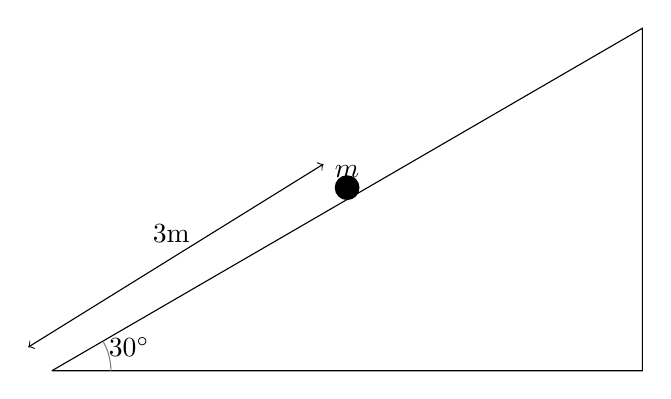
\begin{tikzpicture}[scale=1.5]
	\draw (0,0) -- (5,0) -- (5,2.9) -- (0,0);
	\draw[gray] (0.5,0) arc (0:30:0.5);
	\node[right] at (0.4,0.2) {$30^\circ$};
	\draw[fill] (2.5, 1.55) circle [radius=0.1];
	\node[above] at (2.5,1.55) {$m$};
	\draw[<->] (-0.2,0.2) -- (2.3,1.75);
	\node[above left] at (1.25,1) {3m};
\end{tikzpicture}
\end{center}




\begin{enumerate}
	\item Resolve the gravitational force on the particle into components perpendicular to and parallel to the slope. Draw these on the diagram.
	\item There are two other forces acting on the particle; name them, and give their magnitudes and directions. Draw them on the diagram.
	\item Let $\mu$ be the coefficient of friction of the slope. What inequality must $\mu$ satisfy?
	\item A force is applied to the particle, parallel to the slope and downwards, such that the particle just starts to move. Find the magnitude of this force in terms of $m$ and $\mu$.
	\item Suppose this force is now increased to double its magnitude. How quickly does the particle accelerate?
	\item How long does it take the particle to reach the bottom of the slope?
	\item How quickly is the particle moving when it reaches the bottom?
\end{enumerate}




\clearpage




In the diagram below, two particles, of masses $2m$ and $3m$, as shown, are connected by a light, inextensible string, which passes over a smooth, fixed pulley. The heavier particle starts at the bottom of a ramp, at an angle $\theta$ above the horizontal, with the string running up the ramp and passing over the pulley, so that the lighter particle hangs down.


\begin{center}
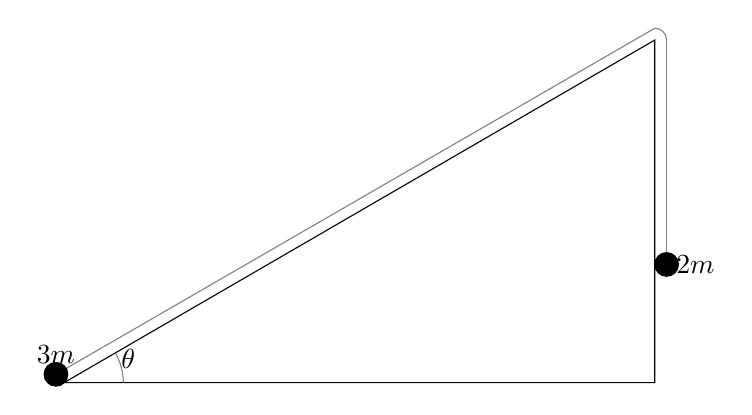
\begin{tikzpicture}[scale=1.5]
	\draw (0,0) -- (5,0) -- (5,2.9) -- (0,0);
	\draw[gray] (0.5,0) arc (0:30:0.5);
	\node[right] at (0.4,0.2) {$\theta$};
	
	\draw[gray] (-0.07,0.07) -- (5,3);
	\draw[fill] (-0.07,0.07) circle [radius=0.1];
	\node[above] at (-0.07,0.08) {$3m$};
	\draw[gray] (5,3) arc (90:0:0.1);
	\draw[gray] (5.1,2.9) -- (5.1,1);
	\draw[fill] (5.1,1) circle[radius=0.1];
	\node[right] at (5.1,1) {$2m$};

\end{tikzpicture}
\end{center}

\begin{enumerate}
	%\item Draw on the diagram the forces acting on both particles.
	% lighter: 2mg down, T up. heavier: 3mg down, T up the slope, R normal to the slope, F either up or down the slope.
	\item Resolve the force of gravity on the heavier particle into components parallel and perpendicular to the slope.
	% 3mg\cos(\theta) into the slope, 3mg\sin(\theta) down the slope.
	\item Suppose the system is at rest. What is the tension in the string?
	% 2mg
	\item Assume the ramp is smooth and the system is at rest. Find $\theta$.
	% the heavier particle has 3mg\sin(\theta)=T=2mg, so \sin(\theta)=2/3, so \theta=\sin^{-1}(2/3)\approx 0.7297
	\item Now assume the ramp has coefficient of friction $0.2$, and $\theta$ is decreased below the value you found above. In what direction does friction act?
	% \theta decreased means smaller force down the ramp, so must have friction acting down the ramp
	\item If we keep decreasing $\theta$ from the value you found above, eventually the system will no longer be at rest. Find the value of $\theta$ at which this happens.
	% at the point of starting to move, F=\mu R; R=3mg\cos(\theta), so F=3\mu mg\cos(\theta), and also weight at 3mg\sin(\theta), vs T=mg up the slope. So 3\mu\cos(\theta)+3\sin(\theta)=1. suppose R\sin(\theta+\alpha)=3\mu\cos(\theta)+3\sin(\theta); then R\sin(\alpha)=3\mu=0.6, R\cos(\alpha)=3$, so $R=\sqrt{0.6^2+3^2}\approx 3.059$, and \tan(\alpha)=0.2, so \alpha=\tan^{-1}(0.2). So 3.059\sin(\theta+\tan^{-1}(0.2))=1. So \theta=\sin^{-1}(1/3.059)-\tan^{-1}(0.2)\approx 0.1356.
\end{enumerate}







\end{document}